% !TeX program = xelatex
% 连续运行两次 XeLaTeX，以生成完整目录和交叉引用。
\documentclass[UTF8,a4paper,zihao=-4,fontset=none]{ctexart}
\usepackage[margin=2.5cm,headheight=16pt]{geometry}
\usepackage{fontspec}
\setmainfont{Latin Modern Roman}
\setsansfont{Latin Modern Sans}
\setmonofont{DejaVu Sans Mono}[Scale=MatchLowercase]
\setCJKmainfont{Noto Serif CJK SC}
\setCJKsansfont{Noto Sans CJK SC}
\setCJKmonofont{Noto Sans Mono CJK SC}
\usepackage{amsmath,amssymb,booktabs,array,longtable,graphicx}
\usepackage{xcolor,fancyhdr,caption,hyperref,fvextra,float,enumitem}
\definecolor{navy}{HTML}{173B59}
\definecolor{softgray}{HTML}{F4F6F8}
\hypersetup{colorlinks=true,linkcolor=navy,urlcolor=navy,citecolor=navy,
  pdftitle={编程作业二：基于解码器的语言模型实验报告},
  pdfsubject={手写因果注意力与 LayerNorm；小模型预训练和约300M模型推理}}
\captionsetup{font=small,labelfont=bf,labelsep=quad}
\ctexset{section={format=\Large\bfseries\sffamily\color{navy}},
  subsection={format=\large\bfseries\sffamily}}
\setlength{\parindent}{2em}
\linespread{1.25}
\setlist{nosep,leftmargin=2em}
\renewcommand{\topfraction}{0.92}
\renewcommand{\bottomfraction}{0.85}
\renewcommand{\textfraction}{0.05}
\renewcommand{\floatpagefraction}{0.8}
\makeatletter
\setlength{\@fptop}{0pt}
\setlength{\@fpsep}{12pt}
\setlength{\@fpbot}{0pt plus 1fil}
\makeatother
\pagestyle{fancy}
\fancyhf{}
\fancyhead[L]{\small 编程作业二：语言模型}
\fancyhead[R]{\small 实验报告}
\fancyfoot[C]{\thepage}
\renewcommand{\headrulewidth}{0.4pt}
\newcommand{\code}[1]{\texttt{\small\detokenize{#1}}}
\DefineVerbatimEnvironment{CodeBlock}{Verbatim}{fontsize=\small,breaklines=true,
  frame=single,rulecolor=\color{gray!40},framesep=2mm}
% Auto-generated from actual results/*.json. Do not edit measured values.
\newcommand{\SmallParams}{3,208,960}
\newcommand{\LargeParams}{302,509,056}
\newcommand{\InitialTrain}{4.2531}
\newcommand{\InitialVal}{4.2551}
\newcommand{\FinalTrain}{1.4649}
\newcommand{\FinalVal}{1.6473}
\newcommand{\InitialPPL}{70.46}
\newcommand{\FinalPPL}{5.19}
\newcommand{\TrainReduction}{65.56}
\newcommand{\ValReduction}{61.29}
\newcommand{\WallSeconds}{91.86}
\newcommand{\SmallMemory}{484.12}
\newcommand{\LargeMemory}{1766.05}
\newcommand{\TrainingTokens}{8,192,000}
\newcommand{\EffectivePasses}{8.16}
\newcommand{\LargeOffset}{0.836}
\newcommand{\LargeSeconds}{2.562}
\newcommand{\LargeSpeed}{31.22}
\newcommand{\LargeProbeLoss}{4.2733}
\newcommand{\LargeParameterMiB}{1153.98}
\newcommand{\FinalGap}{0.1823}
\newcommand{\ExperimentDate}{2026年10月22日}


\begin{document}
\thispagestyle{plain}
\begin{center}
{\small\color{gray} 编程作业二\quad 实验报告}\par
\vspace{0.5em}
{\zihao{2}\bfseries 基于解码器的语言模型}\par
\vspace{0.8em}
{\small 人智2401班}\par
\vspace{0.35em}
{\small
\renewcommand{\arraystretch}{1.2}
\begin{tabular}{@{}l@{\hspace{2.2em}}l@{}}
石皓文\enspace 2233316022 & 张恩瑞\enspace 2244413862\\
杜鹏宇\enspace 2223210437 & 许程\enspace 2244313744
\end{tabular}
}\par
\vspace{0.5em}
{\color{gray!50}\rule{0.92\textwidth}{0.4pt}}
\end{center}
\begin{abstract}
用 PyTorch 基础张量运算实现解码器语言模型，包含因果多头注意力、LayerNorm、可学习位置编码、
残差前馈网络和共享词嵌入的输出头。Tiny Shakespeare 字符语料上的 4 层模型训练 2,000 步后，
训练交叉熵从 \InitialTrain{} 降到 \FinalTrain{}，验证交叉熵从 \InitialVal{} 降到 \FinalVal{}。
24 层配置的参数量为 \LargeParams{}，按要求只做统计和推理。
\end{abstract}
\noindent\textbf{关键词：}解码器语言模型；因果自注意力；LayerNorm；下词预测；参数统计

\section{实验目的}

实现一个 GPT 风格的解码器语言模型，先在 4 层小模型上调试和训练，再统计约 300M 配置的参数并做推理。注意力和 LayerNorm 均由基础运算实现；输入使用字符级编码，文中的“下词”指下一个字符。

\section{模型结构与实现}

\subsection{输入、位置编码与模型输出}
令词表大小为 $V$，批大小为 $B$，序列长度为 $T$，隐藏维度为 $d$。
输入索引 $X\in\{0,\ldots,V-1\}^{B\times T}$，初始表示为
\begin{equation}
H^{(0)}_{b,t}=E[X_{b,t}]+P[t],\qquad
E\in\mathbb{R}^{V\times d},\quad P\in\mathbb{R}^{T_{\max}\times d}.
\end{equation}
位置编码选择可学习的绝对位置嵌入，$T_{\max}=128$。
依次经过 $L$ 个解码器块后，计算
\begin{equation}
Z=\operatorname{LN}(H^{(L)})E^\top\in\mathbb{R}^{B\times T\times V},\qquad
p(x_{t+1}\mid x_{\leq t})=\operatorname{softmax}(Z_t).
\end{equation}
输出 logits 给出每个字符作为下一个词元的得分。
词表输出头与 $E$ 共享同一个参数对象，不额外设置输出偏置。
共享参数既减少规模，也要求统计与优化时避免重复计算。

\subsection{手写因果多头自注意力}
多头结构遵循缩放点积注意力的定义\cite{vaswani2017}。
设注意力头数为 $h$，每头维度 $d_h=d/h$。先用一次基础线性映射产生 $Q,K,V$，
再通过 \code{reshape} 和 \code{transpose} 转成 $[B,h,T,d_h]$。
对每个头计算
\begin{align}
S&=\frac{QK^\top}{\sqrt{d_h}}+M,\\
M_{i,j}&=\begin{cases}0,&j\leq i,\\-\infty,&j>i,\end{cases}\\
A_{i,j}&=\frac{\exp(S_{i,j})}{\sum_{k\leq i}\exp(S_{i,k})},\qquad O=AV.
\end{align}
将各头输出拼接回 $[B,T,d]$，再施加输出投影。掩码在 softmax \textbf{之前}作用，
被屏蔽位置的权重严格为零；保留对角线意味着当前位置可以看到自身的输入词元。
因为训练目标已经右移一位，该操作不会暴露目标词元。
softmax 使用 FP32 计算，再转换回激活数据类型。

核心路径示意如下（代码见 \code{src/model.py}）：
\begin{CodeBlock}
q, k, v = self.qkv(x).chunk(3, dim=-1)
# reshape to [B, T, h, dh], then transpose to [B, h, T, dh]
scores = (q @ k.transpose(-2, -1)) / math.sqrt(self.head_dim)
scores = scores.masked_fill(~mask, -torch.inf)
weights = torch.softmax(scores.float(), dim=-1).to(q.dtype)
heads = self.attention_dropout(weights) @ v
\end{CodeBlock}
这里没有调用现成的多头注意力或 Transformer 模块；注意力矩阵按 $O(BhT^2)$ 的方式直接计算。

\subsection{手写 LayerNorm 与 Pre-LN 解码器块}
对每个词元独立地沿隐藏维度计算
\begin{equation}
\mu=\frac{1}{d}\sum_{i=1}^{d}x_i,\quad
\sigma^2=\frac{1}{d}\sum_{i=1}^{d}(x_i-\mu)^2,\quad
\operatorname{LN}(x)_i=\gamma_i\frac{x_i-\mu}{\sqrt{\sigma^2+\epsilon}}+\beta_i,
\quad\epsilon=10^{-5}.
\end{equation}
方差按 $d$ 取平均，与 LayerNorm 的定义一致。
$\gamma$ 初始化为 1，$\beta$ 初始化为 0；低精度输入的统计量用 FP32 计算。

单个 Pre-LN 块依次计算
\begin{align}
U&=H+\operatorname{Dropout}\bigl(\operatorname{MHA}(\operatorname{LN}_1(H))\bigr),\\
H'&=U+\operatorname{Dropout}\bigl(W_2\operatorname{GELU}(W_1\operatorname{LN}_2(U)+b_1)+b_2\bigr),
\end{align}
其中前馈层先将 $d$ 扩展到 $4d$，再映射回 $d$。注意力概率也施加 dropout。
主体采用 GPT 风格的解码器结构\cite{radford2019}，不包含编码器或交叉注意力。
各矩阵通常以标准差 0.02 的正态分布初始化，两个残差分支的输出投影则使用
$0.02/\sqrt{2L}$，减少深层残差的初始累加幅度。

\subsection{训练目标与自回归生成}
每次从某一数据分区抽取连续 $T+1$ 个词元：前 $T$ 个作为输入，后 $T$ 个作为目标。
例如 \code{abcde} 对应输入 \code{abcd} 和目标 \code{bcde}，模型内部不再次位移。
目标函数为所有位置上的平均负对数似然：
\begin{equation}
\mathcal{L}=-\frac{1}{BT}\sum_{b=1}^{B}\sum_{t=0}^{T-1}
\log p(x_{b,t+1}\mid x_{b,\leq t}).
\end{equation}
生成时只使用最后一个位置的 logits，按温度 $\tau$ 缩放后进行 top-$k$ 采样：
\begin{equation}
p_i=\operatorname{softmax}\left(z_i/\tau\right),\qquad x_{\mathrm{new}}\sim p.
\end{equation}
top-$k$ 以外的 logits 先置为 $-\infty$。输出逐字符拼接，超过 128 个历史字符时保留最近
128 个，并重新从位置 0 编号。生成时关闭 dropout，每次重新计算当前窗口，未使用 KV cache。

\section{数据集、环境与实验设置}

\subsection{数据来源与划分}
采用 Tiny Shakespeare，下载地址见参考文献\cite{tinyshakespeare}。
语料为英文戏剧文本，总计 1,115,394 字节、1,115,394 个字符。
按原始顺序将前 90\%（1,003,854 字符）划为训练段，最后 10\%（111,540 字符）划为验证段。
划分完成后再从各段采样，每个 $T+1$ 窗口都位于同一分区内。
词表仅根据训练段的不同字符构建，大小为 65；验证段不存在训练词表之外的字符。

字符词表保留换行、标点及大小写，不需要单独训练 BPE 分词器。
不过，一个英文单词通常占多个词元，因此 128 个字符能覆盖的文本范围较短。

\subsection{运行环境}

训练使用 Python 3.10.8、PyTorch 2.1.2+cu118、NumPy 1.26.4 和 RTX 3090。随机种子为 42，参数与优化器状态使用 FP32，GPU 前向采用 BF16 autocast。

\subsection{模型与训练超参数}
\begin{table}[htbp]
\centering\small
\caption{模型超参数：小模型训练，大模型仅统计与推理}\label{tab:hyper}
\renewcommand{\arraystretch}{1.1}
\begin{tabular}{lrr}
\toprule
超参数 & 小模型 & 约 300M 模型\\
\midrule
词表大小 $V$ & 65 & 65\\
上下文长度 $T_{\max}$ & 128 & 128\\
解码器层数 $L$ & 4 & 24\\
隐藏维度 $d$ & 256 & 1024\\
注意力头数 $h$ & 4 & 16\\
每头维度 $d_h$ & 64 & 64\\
前馈层维度 $4d$ & 1024 & 4096\\
Dropout & 0.1 & 0（推理）\\
LayerNorm $\epsilon$ & $10^{-5}$ & $10^{-5}$\\
位置编码 & 可学习绝对位置 & 可学习绝对位置\\
输出头权重 & 与词嵌入共享 & 与词嵌入共享\\
实际参数量 & \SmallParams & \LargeParams\\
\bottomrule
\end{tabular}
\end{table}

\begin{table}[htbp]
\centering\small
\caption{小模型训练与评估超参数}\label{tab:trainhyper}
\begin{tabular}{ll}
\toprule
项目 & 设定\\
\midrule
优化器 & AdamW；$\beta_1=0.9,\;\beta_2=0.95,\;\epsilon=10^{-8}$\\
步数与 batch size & 2,000 步；32 个长度为 128 的序列/步\\
学习率 & 前 100 步线性 warmup 至 $5\times10^{-4}$；余弦衰减至 $5\times10^{-5}$\\
权重衰减 & 矩阵参数 0.1；偏置与 LayerNorm 向量 0\\
梯度裁剪 & 全局 $L_2$ 范数上限 1.0；记录裁剪前范数\\
评估 & 第 0 步及每 100 步；每分区固定 16 个 batch\\
评估采样种子 & 训练评估 142；验证评估 242；与训练采样器独立\\
生成所用模型 & 第 2,000 步训练结束时的模型\\
小模型生成 & $\tau=0.8,\;k=20$；三个提示词各生成 240 个字符\\
\bottomrule
\end{tabular}
\end{table}
评估时关闭 dropout，并用固定种子抽取相同窗口。逐步训练损失来自随机 batch，固定窗口损失用于比较训练阶段。

\section{参数统计方法与结果}

\subsection{统计方法}
函数 \code{count_parameters} 遍历命名参数，逐维相乘得到每个张量的元素数，
并用参数对象的 \code{id} 去重，同时保留 \code{lm_head.weight} 等共享别名。
固定因果 mask 是 buffer，不作为可学习参数计入。
根据模型结构，还可以推导参数量公式：
\begin{align}
P_{\mathrm{attn}}&=(3d^2+3d)+(d^2+d)=4d^2+4d,\\
P_{\mathrm{ffn}}&=(4d^2+4d)+(4d^2+d)=8d^2+5d,\\
P_{\mathrm{block}}&=P_{\mathrm{attn}}+P_{\mathrm{ffn}}+4d=12d^2+13d,\\
P_{\mathrm{total}}&=Vd+T_{\max}d+L(12d^2+13d)+2d.
\end{align}
其中 $4d$ 来自块内两组 LayerNorm，末尾的 $2d$ 来自最终 LayerNorm。
共享输出头的 $Vd$ 已在词嵌入中计入。自定义函数、上述公式和 PyTorch 的
\code{model.parameters()} 统计结果一致。

\begin{table}[htbp]
\centering\small
\caption{实际实例化模型的参数统计结果}\label{tab:params}
\begin{tabular}{lrr}
\toprule
模块 & 4 层小模型 & 24 层大模型\\
\midrule
词元嵌入（含共享输出头） & 16,640 & 66,560 \\
可学习位置嵌入 & 32,768 & 131,072 \\
全部解码器块 & 3,159,040 & 302,309,376 \\
最终 LayerNorm & 512 & 2,048 \\
\midrule
总计 & 3,208,960 & 302,509,056 \\
\bottomrule

\end{tabular}
\end{table}
大模型为 \LargeParams{} 参数，即 302.509056M；这里 M 表示 $10^6$。
相对 300,000,000 的偏差为 \LargeOffset\%，符合“约 300M”的规模要求。
FP32 权重本身占 \LargeParameterMiB{} MiB，运行时还需存储激活、中间结果和 CUDA 缓存。

\section{程序调试与结果检查}

调试从 4 层、$d=32$ 的小配置开始，检查各模块的输出和梯度。
测试通过后，将隐藏维度改为 256 进行训练，最后单独运行 24 层大模型的统计与推理。

\subsection{测试项目}

在 $d=32$ 的小配置上检查了七项内容：LayerNorm 的前向值和梯度、因果掩码、整模型因果性、共享权重的参数计数、目标右移、固定小批量过拟合，以及生成时的上下文截断。七项测试均通过。

\subsection{调试过程}
下词预测容易在目标位移上出错，因此先用连续整数序列检查输入和标签，
确认标签只右移一次。注意力部分另写逐头、逐时间位置的循环计算，
与批量矩阵运算对照，检查掩码方向和合头顺序。
还在整个 4 层模型中改动后半段输入，确认前半段 logits 保持不变。

LayerNorm 同时比较前向值和反向梯度，检查均值、方差及可学习参数的计算。
参数统计则重点检查共享输出头，确保它没有和词嵌入重复计数。
小批量过拟合测试中，4 层模型训练 60 步后，损失降到初始值的 10\% 以下，梯度始终有限。
这说明数据、损失函数和优化器已经能够配合工作。
7 项测试全部通过。

正式训练时逐步检查损失和梯度范数；若出现 NaN 或无穷值，程序会停止并报告所在步数。
2,000 步训练没有触发这类异常。

\section{小模型训练结果与分析}

\subsection{训练损失与验证曲线}
表~\ref{tab:loss} 列出几个训练阶段的固定窗口评估结果。
图~\ref{fig:loss} 由训练日志绘制，浅色线是每一步的训练损失，
蓝线和橙线分别是固定训练窗口和验证窗口的交叉熵。

\begin{table}[htbp]
\centering
\caption{固定窗口交叉熵与字符困惑度（交叉熵单位：nat）}\label{tab:loss}
\begin{tabular}{rrrr}
\toprule
优化步 & 训练交叉熵 & 验证交叉熵 & 验证困惑度\\
\midrule
0 & 4.2531 & 4.2551 & 70.46 \\
100 & 2.5058 & 2.5122 & 12.33 \\
500 & 2.0020 & 2.0895 & 8.08 \\
1000 & 1.6636 & 1.8165 & 6.15 \\
1500 & 1.5213 & 1.6964 & 5.45 \\
2000 & 1.4649 & 1.6473 & 5.19 \\
\bottomrule

\end{tabular}
\end{table}

\begin{figure}[htbp]
\centering
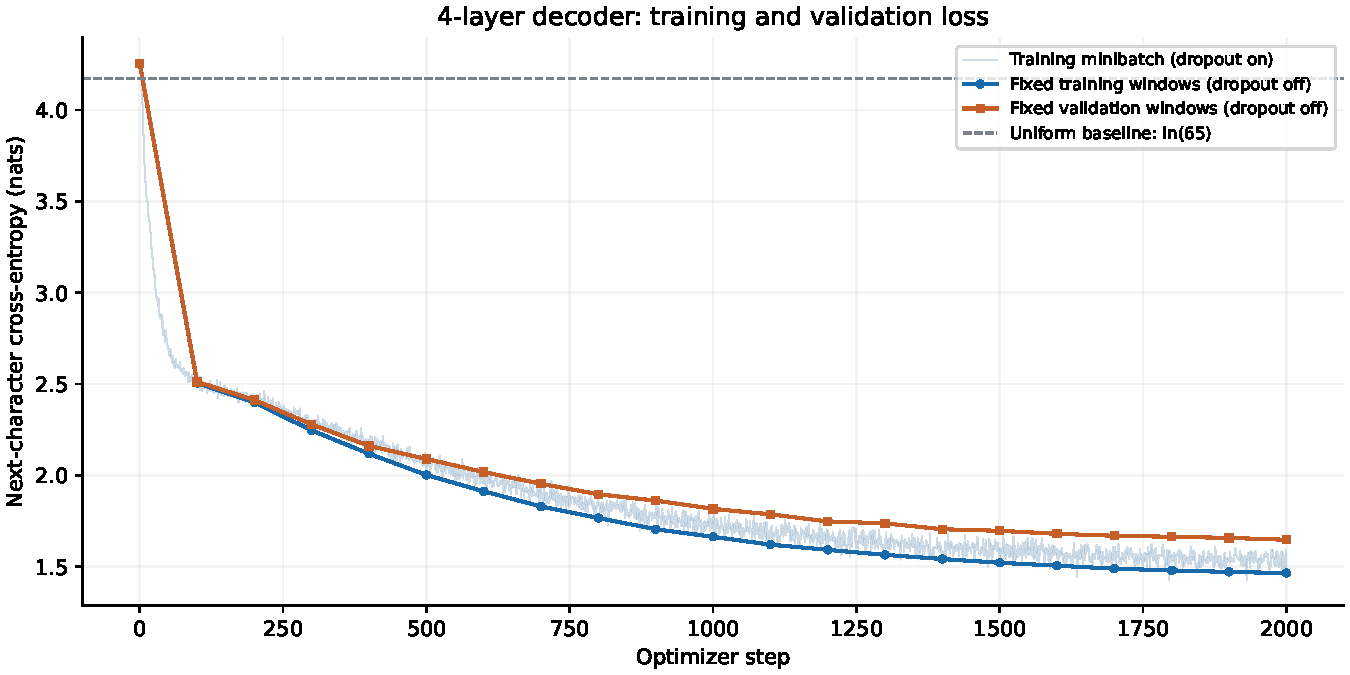
\includegraphics[width=\textwidth]{figures/training_loss.pdf}
\caption{训练与验证损失曲线。虚线表示均匀预测 65 个字符时的交叉熵 $\ln65\approx4.1744$。}\label{fig:loss}
\end{figure}

最终训练交叉熵下降 \TrainReduction\%，验证交叉熵下降 \ValReduction\%，
验证困惑度由 \InitialPPL{} 降至 \FinalPPL{}。
前 100 步下降最快，随后下降速度逐渐放缓。
训练和验证曲线在后期拉开一些距离，最终相差 \FinalGap{} nat，
但验证损失仍在下降，还没有出现明显反弹。
这一结果表明模型已经学到部分字符组合规律；结合后面的生成样例看，语言表达仍有较大改进空间。

\begin{figure}[htbp]
\centering
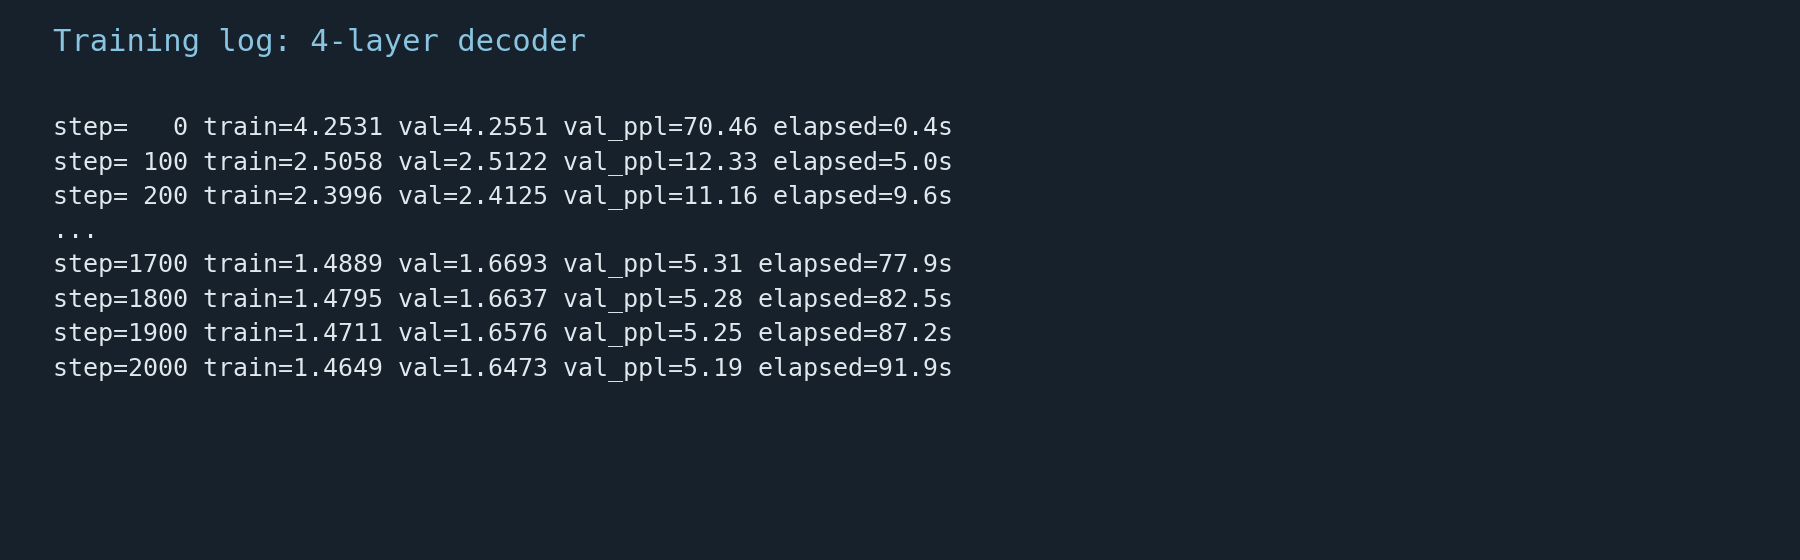
\includegraphics[width=\textwidth]{figures/training_log_excerpt.png}
\caption{训练过程摘录，列出部分步数的损失、困惑度与耗时。}\label{fig:console}
\end{figure}

\section{字符串生成样例}

使用最终权重，分别输入角色名、对白开头和短语进行续写。
三次采样的随机种子为 2026、2027、2028，温度为 0.8，top-$k$ 为 20，各生成 240 个新字符。
下列文本包含提示词，拼写和标点保持生成时的样子。末尾有时在单词中间截断，是固定生成长度所致。

\subsection{样例一：角色名提示}
\begin{Verbatim}[fontsize=\small,breaklines=true,frame=single,framesep=2mm]
ROMEO:
I bid; let my fair son so so, the movery well;
Nor grants a king, ever tower home free;
And come thou did to age it on them,
We the disserve that out not him with thy best,
And thou passit have no from the gentle;
And not of the hearts trob
\end{Verbatim}

\subsection{样例二：对话提示}
\begin{Verbatim}[fontsize=\small,breaklines=true,frame=single,framesep=2mm]
First Citizen:
O, think nevery thou would were to the beath,
And hath sting sent the down of me sink of a
rooth four and do on men can the new-brave work
Ap for the came offends that is stried to was be come
Be his these of their hearts of on't;
I'll suff
\end{Verbatim}

\subsection{样例三：短语续写}
\begin{Verbatim}[fontsize=\small,breaklines=true,frame=single,framesep=2mm]
To be, or not to be and to my come; and well the voy
Be then and friid that the care that a house,
And help liest the reposet my false.

PETRUCKING:
My lord. And their will world, sir; this both these
Shall them should seek me wrong for seems have no me
stas
\end{Verbatim}

输出保留了角色名、换行和对白格式，但拼写和语义仍不稳定。
\section{约 300M 模型的统计与推理演示}

大模型沿用同一个模型类，将配置改为 $L=24,d=1024,h=16$，
参数量为 \LargeParams{}。按作业要求，这一配置只做统计和推理，
权重以种子 300 随机初始化，不进行训练。

\begin{table}[htbp]
\centering\small
\caption{约 300M 模型的推理结果（随机初始化）}\label{tab:large}
\begin{tabular}{ll}
\toprule
项目 & 运行结果\\
\midrule
参数统计结果 & 自定义函数、公式与 PyTorch 均为 \LargeParams\\
完整上下文 logits 形状 & $[1,128,65]$，全部为有限值\\
单窗口下词预测交叉熵 & \LargeProbeLoss{} nat\\
采样设定 & 种子 301；$\tau=1.0$；不做 top-$k$ 截断\\
新增词元数 & 80 个字符\\
生成耗时 / 吞吐量 & \LargeSeconds{} 秒 / \LargeSpeed{} 字符每秒\\
峰值 PyTorch 已分配显存 & \LargeMemory{} MiB\\
权重状态 & 随机初始化，未训练\\
\bottomrule
\end{tabular}
\end{table}

随机初始化模型生成的 80 个字符如下：
\begin{Verbatim}[fontsize=\small,breaklines=true,frame=single,framesep=2mm]
ROMEO:
kA3PMw-x&w CaJEBXOLq.ky-fi.Kr!,,xPF:ZKCsJ,JOlSPakOZmA?S-UgzrrW,Nd:,!XK.rpk,D
$L'
\end{Verbatim}
输出没有连贯含义；这一步只检查大配置的前向计算和采样。

\section{结论}

4 层模型的训练和验证损失都下降，说明手写的注意力、LayerNorm、目标右移和训练流程能够正常工作。24 层配置统计得到 \LargeParams{} 个参数，并完成了按要求的推理演示。生成结果仍有拼写和语义问题，后续可以增加训练步数或改进分词方式。

\begin{thebibliography}{9}
\raggedright
\bibitem{vaswani2017} Vaswani A, Shazeer N, Parmar N, et al.
Attention Is All You Need[C]. NeurIPS, 2017.
\url{https://arxiv.org/abs/1706.03762}.
\bibitem{ba2016} Ba J L, Kiros J R, Hinton G E.
Layer Normalization[EB/OL]. 2016.
\url{https://arxiv.org/abs/1607.06450}.
\bibitem{radford2019} Radford A, Wu J, Child R, et al.
Language Models are Unsupervised Multitask Learners[R]. OpenAI, 2019.
\bibitem{tinyshakespeare} Tiny Shakespeare dataset[DS/OL].
karpathy/char-rnn, data/tinyshakespeare/input.txt.
\url{https://github.com/karpathy/char-rnn/tree/master/data/tinyshakespeare}.
数据下载与实验日期：\ExperimentDate.
\end{thebibliography}
\end{document}
